\documentclass[french,11pt,notitlepage]{report}
\usepackage[utf8]{inputenc}
\usepackage[T1]{fontenc}
\usepackage{lmodern}
\usepackage[a4paper]{geometry}
\usepackage[francais]{babel}
\usepackage{graphicx}
\usepackage{amssymb}
\usepackage{amsmath}
\usepackage{subcaption} 



\begin{document}
	\title{Functional data analysis applied to neurology}
	\author{Clément Bonvoisin, Pierre Ludmann}
	\date{30 juin 2014}
	\maketitle

	\begin{abstract}
  
Il s'agit de segmenter des signaux de marche,
dans le cadre d'une collaboration du CMLA (ENS Cachan) et Cognac-G (Paris V).

On propose donc ici des algorithmes pour détecter des ruptures.
Cela permet en aval aux médecins de mieux étudier les différents régimes de marche.
Un algorithme efficace et rapide semble encore manquer ;
la marche étant souvent abordée sur de longues durées \cite{Was}.

Si la détection d'un unique changement trouve des implémentations reconnues,
on a cherché à généraliser à de multiples ruptures.
Aussi on a changé le paramètre de décision :
on exige un nombre précis de résultats plutôt qu'un seuil de détection.

Malgré de fortes hypothèses de travail,
on obtient des résultats statisfaisants sur des signaux réels et synthétiques
bien que des améliorations restes possibles.

Son utilisation doit faire place à un apprentissage sur les segments de régime obtenus.
	
	\end{abstract}

\phantom{kcahkcah}

\subsection*{Remerciements}

Nous tenions à remercier nos encadrants junior
Emile Contal pour avoir trop souvent fait passer ses stagiaires devant son travail et sa thèse et
Laurent Oudre pour son aiguillage de connaisseur,
nos encadrants seniors Eva Wesfreid et Nicolas Vayatis qui sont à l'origine du sujet de stage.

%\addcontentsline{toc}{subsection}{Remerciements}



	\tableofcontents



	\chapter{Introduction au problème}
	
	
	
	\section{Motivations}
	
	
		La motivation initiale de ce stage provient de la médecine,
		et plus particulièrement de la neurologie.
		Le projet, piloté par le groupe Cognac-G,
		vise à analyser en détail des signaux physiologiques,
		issus d'une expérience très simple.
		Le protocole expérimental se décline comme suit :
		
		On place sur le patient un ensemble de capteurs :
	\begin{itemize}
		\item sur la tête
		\item sur la ceinture, dans le dos
		\item sur chaque pied
	\end{itemize}	
	
		Ces capteurs sont des centrales inertielles, qui permettent une mesure de l'accélération et de la vitesse angulaire du patient.

		On lance alors l'acquisition :
	\begin{itemize}
		\item pendant quelques secondes, le patient est à l'arrêt
		\item puis, il commence à marcher sur une dizaine de mètres
		\item effectue un demi-tour
		\item et fait une marche retour.
	\end{itemize}
		
	Il s'arrête, et on peut alors arrêter l'acquisition.

	\begin{figure}[!h]
		\hspace{5.6cm}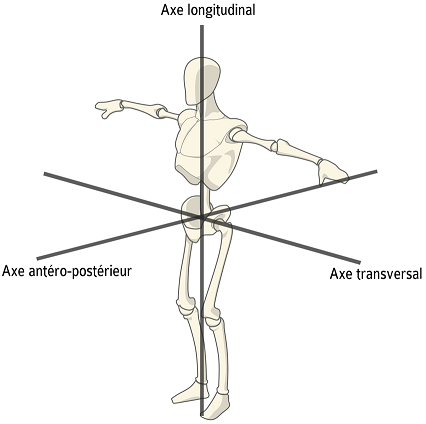
\includegraphics[scale=0.3]{axis.png}
		\caption{Le repère (antéro-postérieur; médio-latéral; vertical)}
		\label{axis}
	\end{figure}
	
	On replace alors les signaux obtenus dans un repère adapté au corps humain, formé de trois axes :
	l'axe antéro-postérieur, l'axe transversal (aussi appelé médio-latéral), et l'axe longitudinal (aussi appelé axe vertical).
		
	\vspace{1pc}
	
	On obtient alors des signaux physiologiques ayant 6 composantes distinctes pour chaque capteur,
	à une fréquence d'acquisition dépendante de la centrale inertielle utilisée ;
	actuellement, le groupe de travail Cognac-G dispose d'instruments permettant un échantillonnage à 100Hz.

% MANQUE DES LABELS
	
	\begin{figure}[!h]
		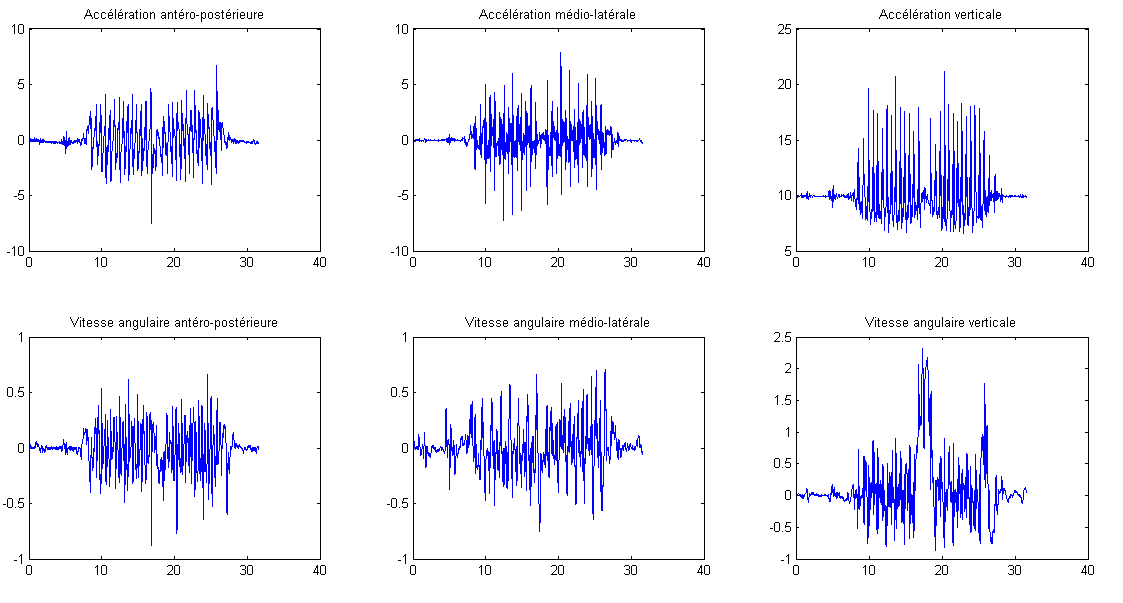
\includegraphics[scale=0.5]{ex_signal_back.png}
		\caption{Un exemple de signal de marche (enregistré à la ceinture)}
		\label{ex_signal_back}
	\end{figure}
	
	Sur ces signaux apparaissent de manière claire les différentes phases de l'expérience :
	\begin{itemize}
		\item Dans un premier temps, le patient est à l'arrêt, les 6 signaux sont quasiment constants (on n'observe que du bruit)
		\item Dans une seconde phase, le patient commence à marcher :
		on peut observer une phase transitoire entre l'arrêt et la marche dite de croisière
		\item La troisième phase de l'expérience correspond à la marche de croisière :
		le patient effectue une dizaine de mètres
		\item On observe ensuite le demi-tour (particulièrement sur les composantes verticales du signal), qui dure environ 1 seconde
		\item Puis, on a une nouvelle phase de marche, retour cette fois-ci
		\item Finalement, le patient s'arrête :
		on a à nouveau une phase transitoire, puis l'arrêt total du patient (où il ne reste plus que du bruit)
	\end{itemize}
	
	\vspace{1pc}
	
	Partant de ceci, on peut donc constater que les signaux acquis par les centrales inertielles peuvent être segmentés,
	qu'on peut isoler les différentes phases de l'expérience.
	Sur un seul signal, cela peut être fait de manière manuelle ;
	néanmoins,
	pour un neurologue enregistrant de manière régulière ce type d'expérience,
	il est concevable de désirer des algorithmes robustes permettant de traiter de manière automatique le problème de la détection des points de changement,
	décomposant ainsi le signal en sous-signaux correspondant à chacune des phases de l'expérience, afin de pouvoir les analyser séparément.
	
	
	\section{Formalisme mathématique}
	
	
	Afin de pouvoir traiter mathématiquement le problème,
	il nous faut tout d'abord poser des définitions claires sur l'objet du problème :
	il s'agit donc de définir ce qu'est une rupture,
	au sens mathématique.
	\\
	
	La littérature propose une approche statistique du problème : 
	on considère les signaux comme la réalisation d'une suite (finie) de variables aléatoires.
%Proposer ici des références bibliographiques...
	\begin{equation}
		(x_i)_{i \in [\![1\,; N]\!]} = (X_i(\omega))_{i \in [\![1\,; N]\!]}
		\label{11}
	\end{equation}
	
	Ce formalisme,
	qui peut paraître quelque peu abstrait en première approche,
	permet d'exprimer de manière simple la notion de rupture dans un signal.
	\\
	
	Sur les signaux précédents, on constate, par exemple,
	une différence nette d'écart-type entre la phase à l'arrêt et la phase de marche ;
	de même, sur la vitesse angulaire verticale, on constate un changement de moyenne entre les phases de marche et le demi-tour.
	Il paraît donc naturel de considérer la distribution statistique des différents points d'un signal multivarié pour formaliser le concept de rupture.
	\\
	
	On comprend alors la définition donnée par la littérature d'un point de rupture à un instant $t_0$ :
	\begin{equation}
	\begin{array}{ll}
			\forall i \in [\![1\,; t_0-1]\!], X_i \sim p_0 \\
			 \forall i \in [\![t_0\,; N]\!], X_i \sim p_1 \\
	\end{array}
	\end{equation}
	%Ref. needed
	
	On généralise de manière évidente au cas de $R$ ruptures aux points $(t_r)_{r \in [\![0\,; n-1]\!]}$ :
	
	\begin{equation}
	\begin{array}{lll}
		~ \forall r \in [\![0\,; R-1]\!], \\
		~ \forall i \in [\![t_{r-1}\,; t_r-1]\!], X_i \sim p_r \\
		( \forall i \in [\![t_r\,; t_{r+1}-1]\!], X_i \sim p_{r+1} )
	\end{array}
	\label{multi_rupt}
	\end{equation}
	
	où l'on a posé : $t_{-1} = 1$ et $t_R = N+1$.
	\\
	
	Ce problème étant formalisé, il s'agit maintenant de trouver des méthodes pour détecter ces points de rupture.
	
	
	
	\chapter{Algorithme CUSUM : résolution du cas d'une seule rupture}
	
	
	
	\section{Principe de l'algorithme CUSUM}
	
	
	L'algorithme CUSUM fut proposé en 1954 par E.S. Page \cite{CIS} ; une methode "en ligne" utilisant un seuil de détection.
	Les signaux étant ici déjà réalisés, on lui préfère son adaptation "hors ligne" \cite{DAC}.
	\\
	
	Dans le formalisme précédent, on conçoit que les méthodes de détection de rupture se fondent sur des outils statistiques.
	L'idée de base de l'algorithme CUSUM hors ligne est la suivante :
	comparer l'hypothèse qu'il existe une rupture dans le signal considéré à l'hypothèse qu'il n'y en a pas.
	L'outil utilisé pour cette comparaison est la notion de vraisemblance.
	Pour simplifier, on fera maintenant l'hypothèse d'indépendance des variables aléatoires $(X_i)_{i \in [\![1\,; N]\!]}$.
	\\
	
	La fonction de vraisemblance quantifie la vraisemblance d'une hypothèse étant donnée une observation.
	Ici, l'observation faite est le signal, qui est la réalisation d'un nombre fini de variables aléatoires.
	On cherche à comparer l'hypothèse $H_t$ qu'à l'instant $t$, il y a une rupture, à l'hypothèse $H_0$ qu'il n'y en a pas dans le signal.
	Les vraisemblances de ces hypothèses sont :
	\begin{equation}
	\begin{array}{ll}
		\forall t \in [\![1\,; N]\!], l(H_t) = \prod_{i = 1}^{t-1} p_0(x_i) \prod_{i = t}^{N} p_1(x_i) \\\\
		\phantom{\forall t \in [\![1\,; N]\!], }l(H_0) = \prod_{i = 1}^N\tilde p(x_i) \\
	\end{array}	
	\end{equation}
	
	Introduisons alors le rapport de vraisemblance des hypothèses :
	\begin{equation}
		\forall t \in [\![1\,; N]\!], \Lambda_t = \frac{l(H_t)}{l(H_0)} = \frac{\prod_{i = 1}^{t-1} p_0(x_i) \prod_{i = t}^{N} p_1(x_i)}{\prod_{i = 1]}^{N} \tilde p(x_i)}
	\end{equation}
	
	Pour simplifier, on fera ici l'hypothèse que nos lois sont issues d'une famille de lois indexée par un paramètre $\theta$ qui vit dans un espace donné.

	On a ainsi :
	
	\begin{equation*}
		p_0 = p_{\theta_0}~;~p_1 = p_{\theta_1}~;~\tilde p = p_{\tilde\theta}
	\end{equation*}
	
	On ne connaît pas, a priori, les paramètres $\tilde\theta$, $\theta_0$ et $\theta_1$.
	Pour les estimer, on va donc utiliser l'estimation du maximum de vraisemblance.
	Il en découle alors la formule suivante, à la base de l'algorithme CUSUM, qui donne le logarithme du rapport de vraisemblance (\textit{log-likelihood ratio}, en anglais) :
	
	\begin{equation}
		\forall t \in [\![1\,; N]\!], L_t=\ln \left[ \frac{\sup_{\theta_0}\left\{ \prod_{i=1}^{k-1} p_{\theta_0}(x_i) \right\} \cdot \sup_{\theta_0} \left\{ \prod_{i = k}^{N}p_{\theta_0}(x_i) \right\}}{\sup_{\tilde\theta}\left\{\prod_{i=i}^{N}p_{\tilde{\theta}}(x_i)\right\}} \right]
		\label{log_likelihood_ratio}
	\end{equation}
	
	Finalement, l'instant où il est le plus probable de trouver une rupture est celui qui maximise $L_t$.
	Ainsi, l'estimateur du maximum de vraisemblance (\emph{maximum likelihood estimator}) par CUSUM du point de rupture d'un signal est :
	
	\begin{equation}
		\hat{t_0}=\arg\max_{1\le t\le N}L_t
	\end{equation}
	
	
	\section{Simplification dans le cas de distributions gaussiennes}

	
	Dans le cas général, la formule \ref{log_likelihood_ratio} est peu exploitable en raison de la présence de bornes supérieures.
	Afin de simplifier le problème des estimateurs au maximum de vraisemblance
	, on peut se proposer de faire une hypothèse sur la famille de lois $(p_\theta)_{\theta \in \mathbb{R}^d}$.
	\\
	
	On suppose donc, à partir de maintenant, que chacune des variables aléatoires qui composent le signal suit une loi gaussienne, \emph{i.e.} :
	
	\begin{equation*}
		p_{\mu, \sigma}(y) = \frac1{\sigma\sqrt{2 \pi}} \exp \left[ -\frac12 \left( \frac{y - \mu}{\sigma} \right)^2 \right]
	\end{equation*}
	
	Les estimateurs aux maximas de vraisemblance de la loi normale sont alors connus \cite{MLE}.
	Ceci nous permet alors de simplifier l'expression de $L_t$
	car les bornes supérieures sont atteintes par ces estimateurs.
	Notons que l'hypothèse du gaussien ramène le problème du changement de loi à trois cas : changement de moyenne, changement d'écart-type, et changement de moyenne et d'écart-type.
	\\ \\
	Dans le cas d'un signal multi-varié, on peut généraliser aisément tout ce qui a été dit précédemment en faisant l'hypothèse d'indépendance des différentes composantes du signal entre elles. On calcule alors les \textit{log-likelihood ratios} des différentes composantes du signal indépendamment avant de les additionner, et de chercher le maximum de cette résultante. Tout du long, en vertu de cette remarque, on ne théorisera que le cas univarié.
	\\ \\
	
		Bien que nous n'allons pas immédiatement traîter les signaux physiologiques vus précédemment --
	ceux-ci comportent plusieurs ruptures, l'algorithme CUSUM ne permettant d'en détecter qu'une seule -- il est de bon ton de joindre des exemples imagés à ce flot de formules.
	Les signaux utilisés dans cette partie sont des signaux synthétiques, obtenus grâce à MATLAB.
	
		Aussi les détails et preuves de cette simplification se trouvent en annexe.
		
	
	\subsection{Changement en moyenne}
	
	
	Faisant l'hypothèse d'un écart-type constant sur l'ensemble du signal, le paramètre $\theta$ est ici uniquement la moyenne $\mu$.
	
	\ref{log_likelihood_ratio} se réécrit donc après calculs :
	\begin{equation}
		\forall t \in [\![1\,; N]\!], L_t = \frac{1}{2 \sigma ^2}\left[(t-1)\hat{\mu_0}^2 + (N - t + 1)\hat{\mu_1}^2 - N\hat{\tilde\mu}^2 \right]
		\label{meanchange}
	\end{equation}
	
	$\sigma$ étant donc fixé au préalable. Et $\hat{\tilde\mu}$, $\hat\mu_0$ et $\hat\mu_1$ sont les estimateurs $\hat\mu=\frac1n\sum_{i=1}^nx_i$ du signal respectivement de 1 à $N$, de 1 à $t-1$ et de $t$ à $N$.
	\\
	
	On se place dans le cas d'un changement en moyenne de $\mu_1 = 10$ à $\mu_2 = 20$, avec $t_0 = 201$.
	
	On utilise cette fois l'équation \ref{meanchange} pour obtenir la figure \ref{llr_test_mean}.


	\begin{figure}[h]	
		\begin{subfigure}[t]{.49\textwidth}

  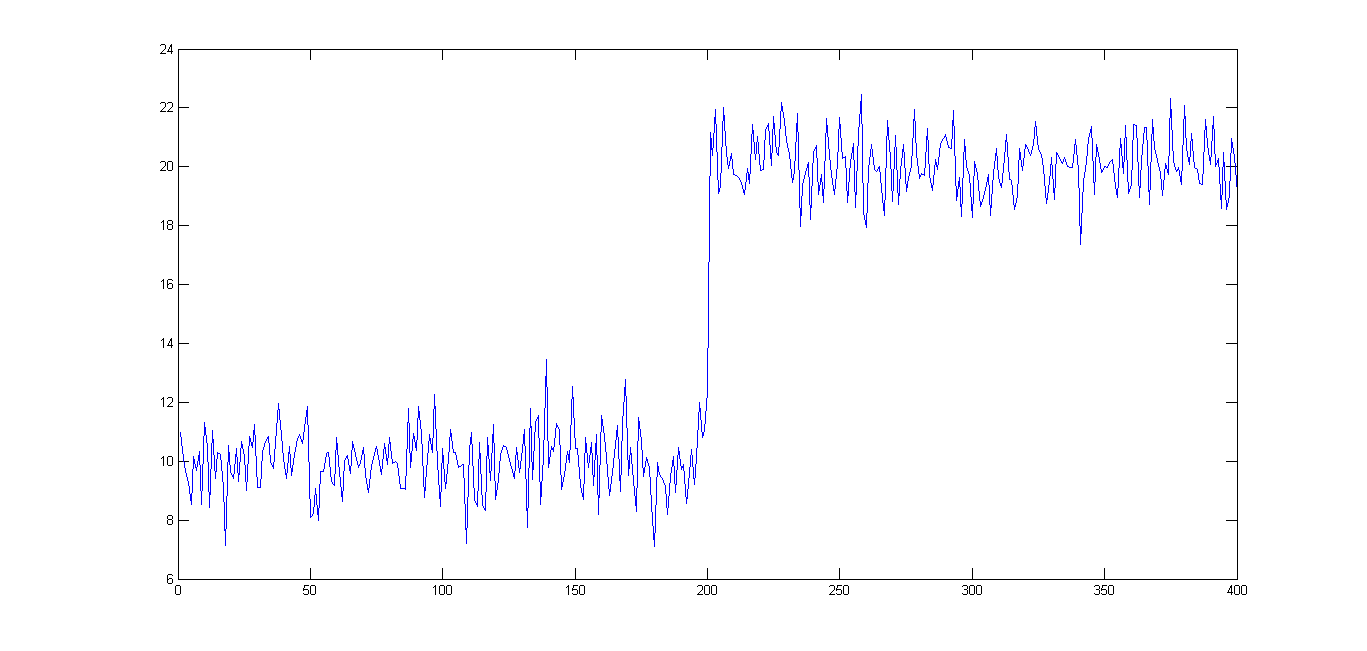
\includegraphics[width=\linewidth]{test_signal_mean.png}
		\caption{Pour $t \leq 200$, $X_t \sim \mathcal{N}(10, 1)$ ; pour $t > 200$, $X_t \sim \mathcal{N}(20, 1)$}
		\label{test_signal_mean}
	\end{subfigure}
	\hfill
	\begin{subfigure}[t]{.49\textwidth}

  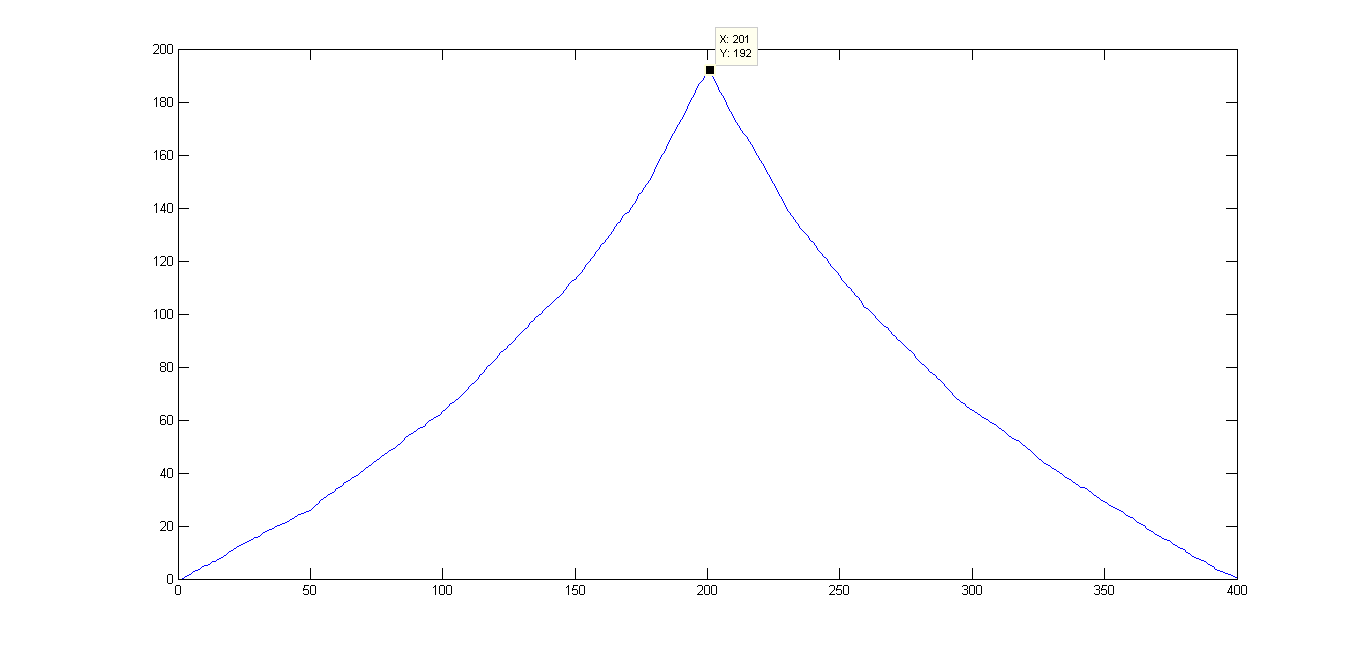
\includegraphics[width=\linewidth]{llr_test_mean.png}
		\caption{\textit{Log-likelihood ratio} du signal précédent}
		\label{llr_test_mean}
	\end{subfigure}
	
	\caption{Exemple de détection d'une rupture par la moyenne}
	\end{figure}
	
	On obtient donc ici l'estimateur du point de rupture par CUSUM, avec un score de 192 :
	\begin{equation*}
		\hat{t_0} = 201 ; \hat{t_0} - t_0 = 0
	\end{equation*}
	
	De même que dans le cas précédent, on observe la robustesse de l'estimateur par CUSUM du point de rupture de ce signal. Pour quantifier cette robustesse, on peut s'appuyer sur la déviation quadratique moyenne de cet estimateur (RMSD), en répétant 5.000 fois l'expérience précédente, on trouve : $RMSD = 0$.
	
	
	\subsection{Changement en écart-type}
	
	
	Faisant cette fois l'hypothèse d'une moyenne constante sur l'ensemble du signal, le paramètre $\theta$ est ici uniquement l'écart-type $\sigma$.
	
	\ref{log_likelihood_ratio} se réécrit alors : 
	
	\begin{equation}
		\forall t \in [\![1\,; N]\!], L_t = N\ln (\hat{\tilde\sigma}) - (t-1)\ln (\hat{\sigma_0}) - (N-t+1)\ln (\hat{\sigma_1})
		\label{stdchange}
	\end{equation}
	$\mu$ étant préalablement fixé. Et $\hat{\tilde\sigma}$, $\hat\sigma_0$ et $\hat\sigma_1$ sont les estimateurs $\hat\sigma=\sqrt{\frac1n\sum_{i=1}^n(x_i-\mu)^2}$ du signal respectivement de 1 à $N$, de 1 à $t-1$ et de $t$ à $N$.
	\\
	
		On se place dans le cas d'un changement en écart-type de $\sigma_0 = 1$ à $\sigma_1 = 3$, à l'instant $t_0 = 201$.
	

	
	\begin{figure}[h]

	\begin{subfigure}[t]{.49\textwidth}

  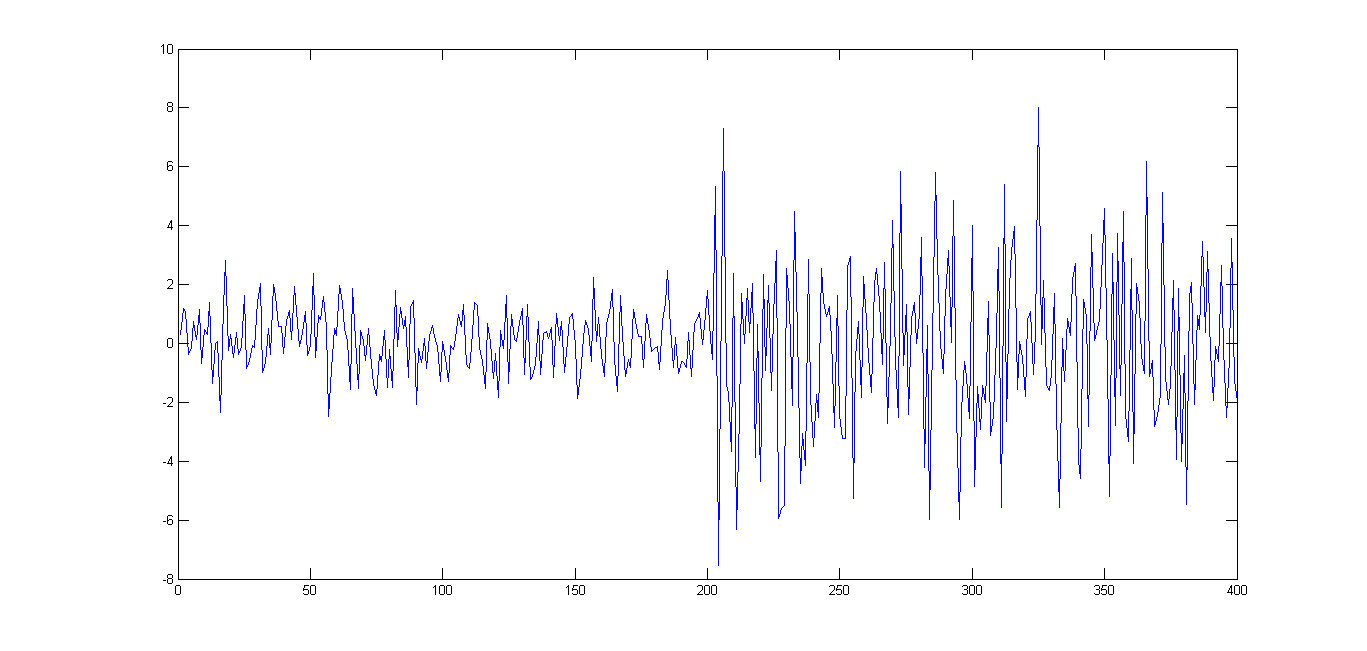
\includegraphics[width=\linewidth]{test_signal_std.png}
		\caption{Pour $t \leq 200$, $X_t \sim \mathcal{N}(0, 1)$ ; pour $t > 200$, $X_t \sim \mathcal{N}(0, 3)$}
		\label{test_signal_std}
	\end{subfigure}
	\hfill
	\begin{subfigure}[t]{.49\textwidth}

  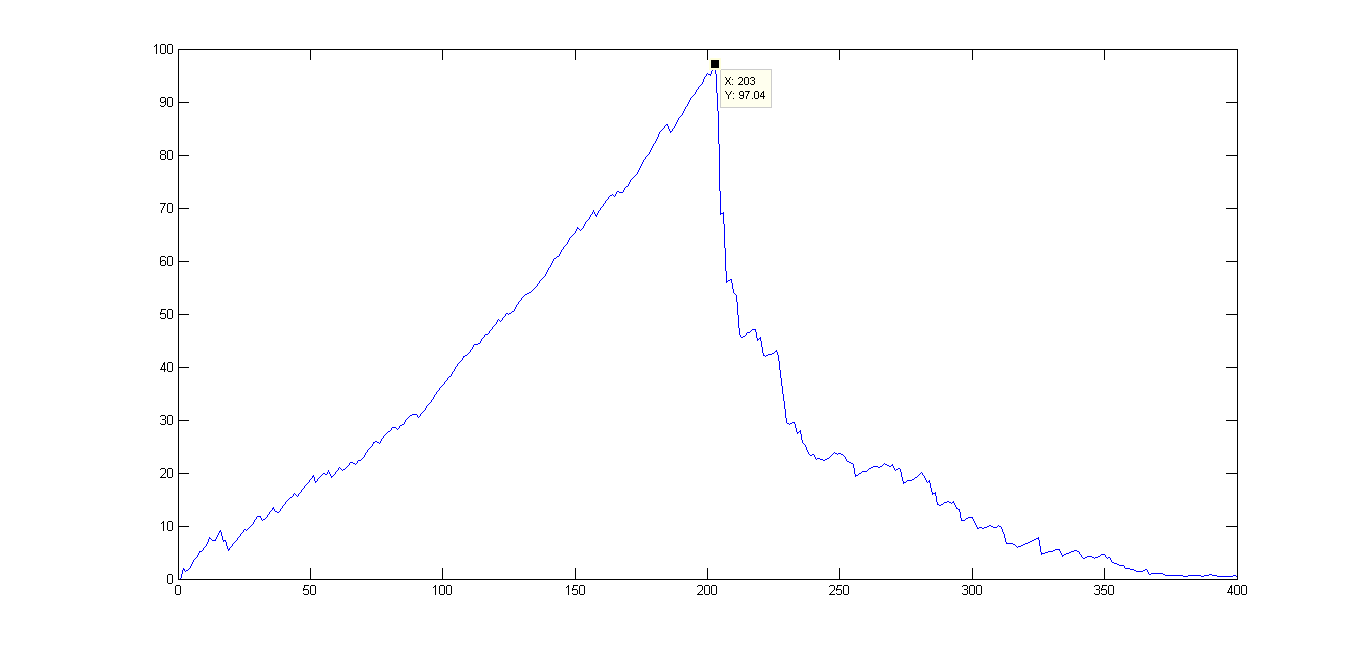
\includegraphics[width=\linewidth]{llr_test_std.png}
		\caption{\textit{Log-likelihood ratio} du signal précédent}
		\label{llr_test_std}
	\end{subfigure}
	\caption{Exemple de détection d'une rupture par l'écart-type}
	\end{figure}
	

	
	L'équation \ref{stdchange} permet alors d'obtenir la figure \ref{llr_test_std}
		
	Ce comportement est le comportement typique de la courbe d'un \textit{log-likelihood ratio} sur un signal gaussien comportant une rupture. On observe ici que le maximum de la courbe est à l'instant 203, avec un \textit{log-likelihood ratio} $L_{203} = 97,04$. On a donc l'estimateur par CUSUM du point de rupture :
	\begin{equation*}
		\hat{t_0} = 203 ; \hat{t_0} - t_0 = 2;
	\end{equation*}
	
	Ainsi, l'estimateur de points de rupture par CUSUM semble robuste dans le cas d'un changement par écart-type. Pour 5.000 signaux différents suivant les caractéristiques précédentes, on trouve : $RMSD = 2,605$.
	
	
	\subsection{Changement en moyenne et en écart-type}
	
	
	Dans ce dernier cas, on doit estimer à la fois la moyenne et l'écart-type des différentes portions du signal. On obtient un résultat quasiment identique à \ref{stdchange} :
	\begin{equation}
		\forall t \in [\![1\,;N]\!], L_t = N\ln (\hat{\tilde\sigma}) - (t-1) \ln (\hat\sigma_0) - (N - t + 1) \ln (\hat\sigma_1)
		\label{bothchange}
	\end{equation}
	La seule différence intervient dans l'estimateur de l'écart-type :
	au lieu d'utiliser une moyenne fixée sur l'ensemble du signal (ce qui peut se traduire légitimement par son estimateur sur la globalité du signal),
	on utilise ici les estimateurs  de la moyenne sur les différentes portions du signal :
	
	$\hat{\tilde\mu}$, $\hat\mu_0$ et $\hat\mu_1$ sont les estimateurs $\hat\mu=\frac1n\sum_{i=1}^nx_i$ du signal respectivement de 1 à $N$, de 1 à $t-1$ et de $t$ à $N$.
	Et $\hat{\tilde\sigma}$, $\hat{\sigma_0}$ et $\hat\sigma_1$ sont les estimateurs $\hat\sigma=\sqrt{\frac1n\left[\sum_{i=1}^nx_i^2-(\sum_{i=1}^nx_i)^2\right]}$ du signal respectivement de 1 à $N$, de 1 à $t-1$ et de $t$ à $N$.	

	
	
	\chapter{Cas de plusieurs ruptures : implémentation dichotomique}
	Nous allons à présent nous intéresser au problème que l'on cherche à résoudre, à savoir celui d'un signal avec plusieurs ruptures. Voyons ici une première approche, qui semble particulièrement intuitive, à savoir l'approche dichotomique.

	\section{Principe théorique}
	Nous allons ici reprendre le principe de l'algorithme CUSUM tel qu'il est décrit dans le chapitre 2, et l'adapter au cas de plusieurs ruptures.
	\\ \\
	Le principe de la dichotomie est simple : à chaque étape de la dichotomie, on compare l'hypothèse qu'il y a une rupture dans le signal à l'hypothèse qu'il n'y en a pas. Il nous faudra ensuite comparer ces ruptures pour en choisir une. Voyons cela plus en détail.
	\\ \\
	À la première étape de la dichotomie, on applique l'algorithme CUSUM classique à notre signal tout entier. Notons qu'on ne cherche pas à valider l'hypothèse qu'il y a une rupture dans le signal, mais qu'on cherche bien à trouver l'instant où cette hypothèse est la plus vraisemblable : on conçoit donc que même si l'hypothèse est fausse (puisqu'il y a plusieurs ruptures dans le signal), son maximum de vraisemblance constituera un bon estimateur pour l'une des ruptures du signal. On a ainsi détecté une rupture, $\hat{t_0}$.
	\\ \\
	On peut alors séparer le signal en deux sous-signaux : $(X_t)_{t \in [1, \hat{t_0}-1]}$ et $(X_t)_{t \in [\hat{t_0}, N]}$. Sur chacun de ces sous-signaux, on peut alors à nouveau effectuer l'algorithme CUSUM, et détecter ainsi deux nouveaux maximas de vraisemblance, que l'on notera $t_{1,1}$ et $t_{1,2}$, associés aux \textit{log-likelihood ratios} $L_{t_{1,1}}^1$ et $L_{t_{1,2}}^2$. On peut alors comparer ces deux \textit{log-likelihood ratios} et en déduire la rupture la plus vraisemblable : si $L_{t_{1,1}}^1 > L_{t_{1,2}}^2$, on considère $\hat{t_1} = t_{1,1}$ ; sinon, on considère $\hat{t_1} = t_{1,2}$.
	\\ \\
	Considérons qu'on est dans le premier cas ici (le second se traite de manière analogue). On peut alors à nouveau découper en deux sous-signaux : $(X_t)_{t \in [1, \hat{t_1}-1]}$ et $(X_t)_{t \in [\hat{t_1}, \hat{t_0}-1]}$. On peut à nouveau déterminer les maximas de vraisemblance de chaque côté, et obtenir ainsi deux instants $t_{2,1}$ et $t_{2,2}$, associés aux \textit{log-likelihood ratios} $L_{t_{2,1}}^2$ et $L_{t_{2,2}}^2$. On compare alors entre eux les \textit{log-likelihood ratios} $L_{t_{2,1}}^2$, $L_{t_{2,2}}^2$ et $L_{t_{1,2}}^1$. Le plus élevé de ces trois, disons $L_{t_{1,2}}^1$ par exemple, permet de sélectionner la rupture suivante : ce sera ici $\hat{t_2} = t_{1,2}$.
	\\ \\
	On redécoupe alors le signal à partir de la dernière rupture observée : ici, on découpe $(X_t)_{t \in [\hat{t_0}, N]}$ en $(X_t)_{t \in [\hat{t_0}, \hat{t_2}-1]}$ et $(X_t)_{t \in [\hat{t_2}, N]}$, et on réapplique l'algorithme CUSUM de chaque côté, en comparant à chaque fois tous les maximas qui n'ont pas été sélectionnés. On répète cette opération jusqu'à avoir le nombre $n$ de ruptures voulu.

	\section{Implémentation algorithmique}


	Nous avons déjà présenté, dans le premier chapitre, le formalisme statistique associé au cas de plusieurs ruptures dans un signal en \ref{multi_rupt}.
	L'implémentation dichotomique du CUSUM consiste alors à calculer un arbre de la façon suivante :
	\\
	\begin{itemize}
	\item Maintenir un ensemble de ruptures choisis initialement vide (les noeuds intérieurs).
	\item Maintenir un ensemble de ruptures éligibles qui contient initialement le résultat du CUSUM sur le signal entier (la frontière, les feuilles).
	\item En extraire la rupture $t_0$ qui a le plus grand ratio de vraissemblance.
	\item Calculer les deux ruptures -- qui sont alors éligibles -- en applicant le CUSUM entre la rupture choisie précédant chronologiquement $t_0$ et $t_0$ et entre $t_0$ et la rupture choisie suivant chronologiquement $t_0$.
	\item Recommencer jusqu'à obtenir le nombre désiré de ruptures.\\
	\end{itemize}
	
	
	Procéder par dichotomie permet d'aller très rapidement dans le traitement : la complexité d'un CUSUM est linéaire en la taille du signal à traiter, on se retrouve dans le pire des cas avec une complexité en $\mathcal O(NR)$ avec $N$ la taille du signal et $R$ le nombre de rupture.
	\\
	
	Mais remarquons que ce n'est pas nécessairement la première approche dichotomique qu'on pourrait envisager.
	Une version plus naïve serait de calculer un arbre de dichotomie complet de taille le nombre de ruptures directement -- en retirant les moins bonnes si surplus.
	C'est en tout cas plus évident que d'aller faire éclore la meilleure de feuille de l'arbre de travail à chaque tour de boucle.
	
	Sauf que l'arbre complet tombe dans un grave écueuil : plusieurs de ses sous-arbres sera vite confiné à calculer des ruptures là où elles sont minimes.
	Par exemple si la racine correspond à la rupture de début de marche tout le sous-arbre de son fils gauche va pointer sur des ruptures dans le régime immobile.
	\\
	
	On pourrait être tenter de remplacer la demande de taille par la demande de profondeur.
	Et on choisirait les $R$ meilleurs ruptures parmi les $2^R$ de l'arbre complet.
	Mais le souci vient alors de cette possibilité, réel, de choisir une rupture sans choisir ses ancestres \emph{i.e.}
	choisir une rupture sans dire que la part de signal qui à permit de la choisir commence et finissent à de bons instants.
	Car si on ne choisit pas ses ruptures parentes c'est bien qu'on considère ce début et cette fin comme n'étant pas significatives.
	\\
	
	Cependant même la dichotomie par la frontière déborde du cadre théorique et principalement près la racine de l'arbre :
	on place une rupture non pas entre deux régimes mais entre plusieurs régimes de part et d'autre de cette rupture.
	Par exemple sur un signal physiologique de marche où le protocole expérimental donne lieu à un minimum de 5 régimes (Idle, Walk, Turn, Walk, Idle) et donc de 4 ruptures :
	même si la première rupture calculée est au bon endroit -- sur un changement de régime --
	elle va en séparer 1 de 4, 2 de 3, 3 de 2 ou 4 de 1.
	On est bien loin du cadre théorique.
	
	
	
	\chapter{Cas de plusieurs ruptures : implémentation par fenêtres}	
	
	
	
	Il a été vu dans la partie précédente que l'implémentation dichotomique du CUSUM débordait du cadre théorique :
	en effet, on fait à itération l'hypothèse d'une unique rupture dans le signal, alors que l'on désire en détecter plusieurs.
	De plus, on cherche dans cette approche à comparer entre elles des ruptures sur des signaux qui n'ont a priori aucun rapport les uns les autres.
	Pour pallier ce défaut, nous proposons ici une approche par fenêtres.
	
	
	\section{Principe théorique}
	
	
	L'algorithme CUSUM, tel qu'il est présenté dans le chapitre 2, ne permet de détecter qu'une seule rupture dans un signal donné.
	Nous traitons ici le cas de signaux ayant un nombre $R$ de ruptures, avec $R \geq 1$.
	Si l'on désire se servir de l'algorithme CUSUM, pour rester dans le cadre théorique,
	il nous faudra nous assurer que le signal qu'on observe ne possède qu'une seule rupture.
	\\
	
	Pour cela, en gardant les notations du chapitre 1, supposons que l'on dispose de l'écart minimal entre deux ruptures :
	\begin{equation*}
		p = \min_{-1 \leq r \leq R-1} (t_{r+1} - t_r)
	\end{equation*}
	
	Ainsi, pour $t \in [p+1, N-p]$, on est assuré d'avoir au plus une rupture dans l'intervalle $[t-p, t+p]$. On peut donc appliquer l'algorithme CUSUM sur des fenêtres centrées en $t$ et de taille $2p+1$. Le principe de l'implémentation par fenêtres est alors d'appliquer l'algorithme CUSUM sur chacun des intervalles $[t-p,t+p]$ pour $t \in [p+1, N-p]$, et de sélectionner ensuite les $R$ meilleures ruptures.
	\\
	
	Pour réduire le problème, simplifions quelque peu l'algorithme CUSUM : on considère ici uniquement l'hypothèse d'une rupture à la date t. On a ainsi, pour $t \in [t-p,t+p]$, deux hypothèses :
	\begin{equation*}
			H_0^t : \forall i \in [t-p, t+p], X_i \sim p_{\tilde{\theta}}
	\end{equation*}
	\begin{equation*}
			H_1^t : 
			\left\{ \begin{array}{ll}
				\forall i \in [t-p, t-1], X_i \sim p_{\theta_0} \\ \forall i \in [t, t+p], X_i \sim p_{\theta_1} \\
			\end{array} \right.
	\end{equation*}
	
	Il s'agit alors, comme c'est fait dans l'algorithme CUSUM pour une rupture, de comparer ces deux hypothèses, ceci pour tout $t$ :
	
	\begin{equation}
		L_t = \ln \left[ \frac{\prod_{i = t-p}^{t-1} p_{\hat{\theta_0}}(x_i) \prod_{i = t}^{t+p} p_{\hat{\theta_1}}(x_i)}{\prod_{i = t-p}^{t+p} p_{\hat{\tilde{\theta}}}(x_i)} \right]
	\end{equation}
	
	Cette formule se simplifie de la même manière que ce qui a été fait dans le chapitre 2, selon les différents types de changement :
	en moyenne, en écart-type, ou les deux en même temps. 
	On cherche alors à sélectionner les $R$ instants où il est le plus vraisemblable de trouver une rupture,
	c'est-à-dire les $R$ plus grands maximas locaux de la suite $(L_t)_{t\in[p+1, N-p]}$.
	
	\section{Implémentation algorithmique}
	Le principe théorique de la détection de ruptures par fenêtres éclaire sur la manière d'implémenter l'algorithme. Pour cela, il nous faut :
	\begin{itemize}
		\item Calculer les scores $L_t$ selon la formule 4.3 après simplification (selon qu'on cherche un changement en moyenne, en écart-type, ou les deux)
		\item Déterminer $\hat{t_0} = \arg \max_{t \in [p+1, N-p]} L_t$
		\item Considérant $\hat{t_0}$ comme une rupture, on sait qu'il n'y a pas d'autre rupture dans la fenêtre $[\hat{t_0}-p, \hat{t_0}+p]$ par hypothèse ; on peut donc retirer de la suite $(L_t)$ les valeurs $(L_t)_{t \in [\hat{t_0}-p, \hat{t_0}+p]}$
		\item On recommence alors sur la sous-suite ainsi obtenue, jusqu'à avoir $n$ ruptures
	\end{itemize}
	
	Observons en détails la manière de procéder sur un exemple (signal \ref{test_multi_rupt})
	\begin{figure}[h]
		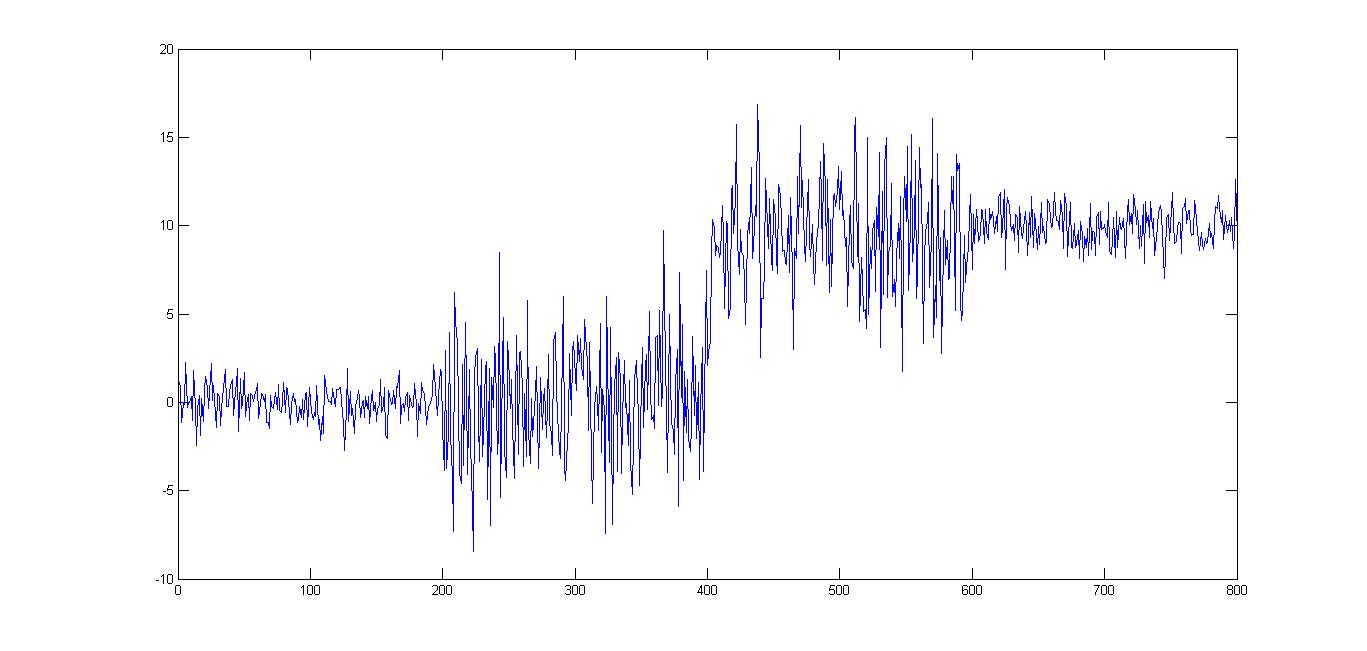
\includegraphics[scale=0.4]{test_multi_rupt.png}
		\caption{De 1 à 200 : $\mathcal{N}(0,1)$ ; de 201 à 400 : $\mathcal{N}(0,3)$ ; de 401 à 600 : $\mathcal{N}(10,3)$ ; de 601 à 800 : $\mathcal{N}(10,1)$}
		\label{test_multi_rupt}
	\end{figure}
	On peut ici assurer un intervalle entre deux ruptures de 200 points (dans la pratique, il faut estimer cet intervalle). Pour pouvoir observer ce qui se passe avant la première rupture et après la dernière, on prendra ici des fenêtres de 150 points de chaque côté. On travaille de plus avec des ruptures en moyenne et en écart-type. On obtient alors la suite $(L_t)$ montrée sur la figure \ref{multi_rupt_llr_ex}.
	
	\begin{figure}[h]
		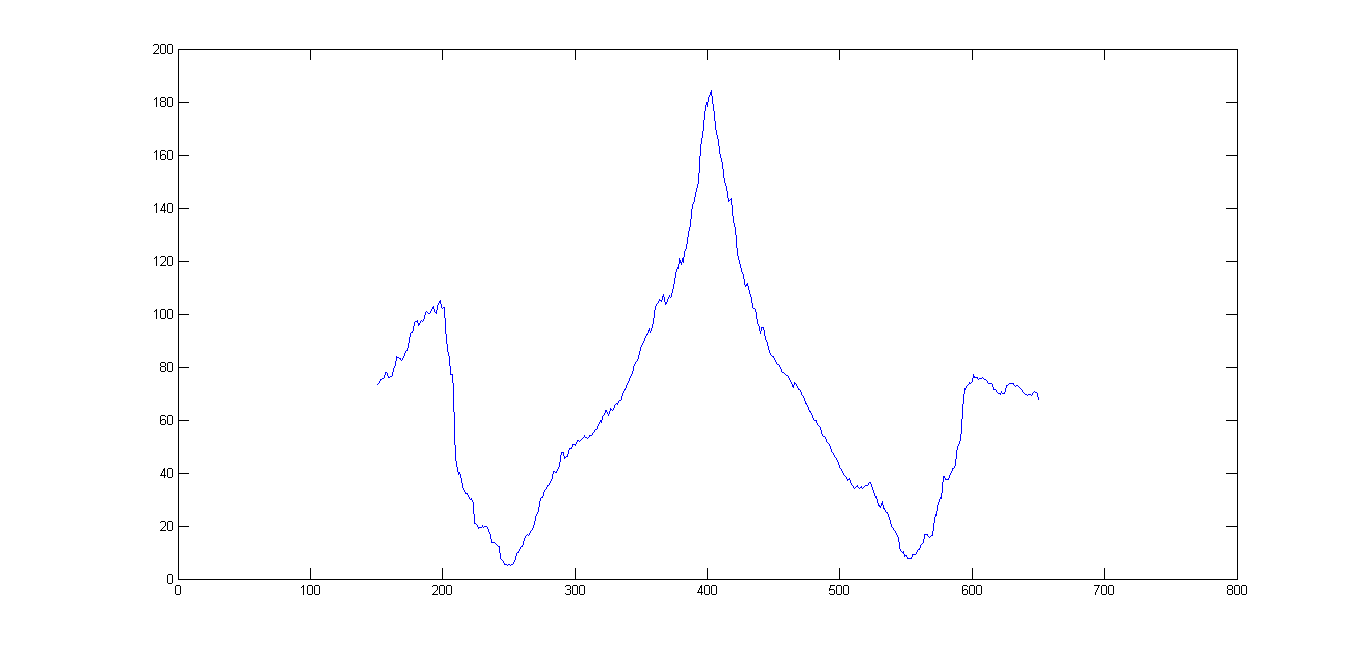
\includegraphics[scale=0.4]{multi_rupt_llr_ex.png}
		\caption{Suite $(L_t)_{t\in[151,650]}$}
		\label{multi_rupt_llr_ex}
	\end{figure}
	
	On demande alors à trouver 3 ruptures à partir de cette figure. On commence par détecter le maximum à $\hat{t_0} = 403$, où $L_{\hat{t_0}} = 184,2725$. On exclut alors les valeurs de $L_t$ pour $t \in [253, 553]$. On cherche alors le nouveau maximum : on trouve $\hat{t_1} = 198$ pour $L_{\hat{t_1}} = 105,1670$. On recommence alors la procédure d'exclusion des points dans le voisinage de cette rupture, et on trouve le dernier maximum : $\hat{t_2} = 601$ pour $L_{\hat{t_2}} = 77,0389$. La segmentation obtenue est montrée sur la figure \ref{test_multi_rupt_seg}.
	
	\begin{figure}[h]
		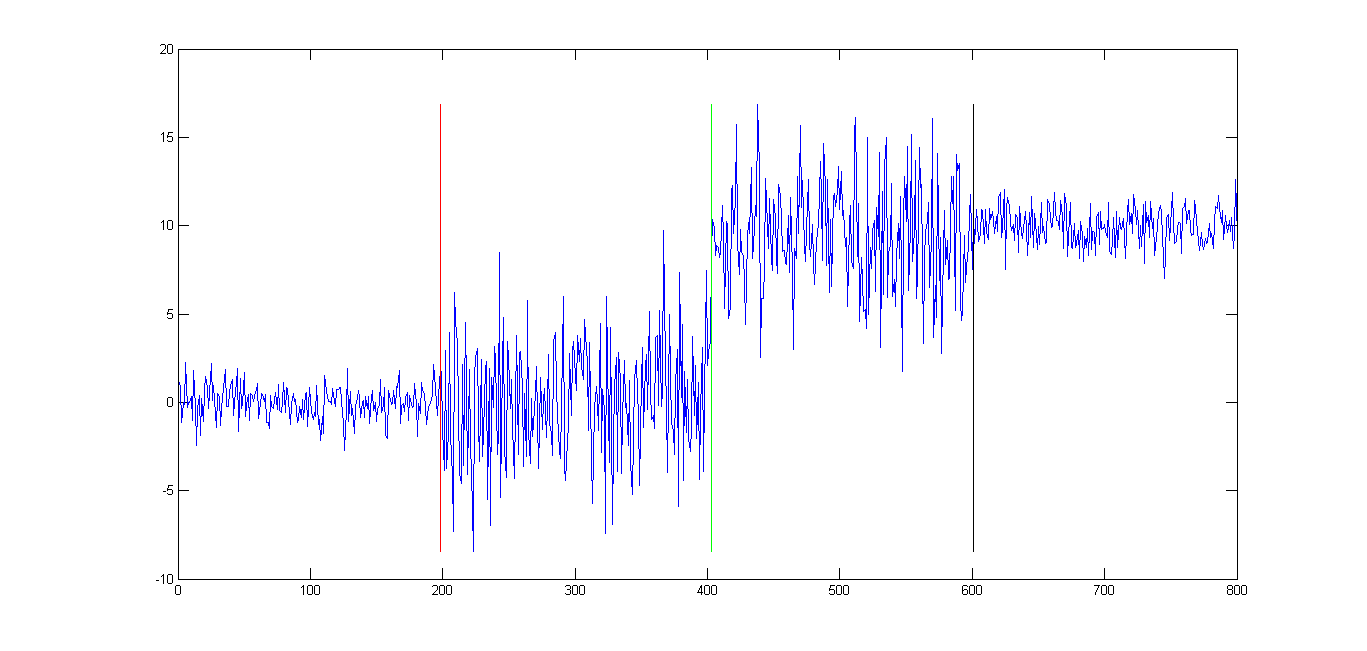
\includegraphics[scale=0.4]{test_multi_rupt_seg.png}
		\caption{Signal segmenté par la méthode par fenêtres ; en vert : rupture 1 ; en rouge : rupture 2 ; en noir : rupture 3}
		\label{test_multi_rupt_seg}
	\end{figure}
	
	\chapter{Évaluation des performances}
	
	
	
	\section{Sur des signaux synthétiques}
	
	Ces signaux sont générés en jouant sur 3 critères :
	
	\begin{itemize}
	\item le nombre de ruptures
	\item l'espace moyen entre les ruptures
	\item l'espace minimal entre mes ruptures\\
	\end{itemize}
	
	Les valeurs de l'espace entre ruptures sont tirés uniforment sur l'intervalle ouvert de $\mathbb R^{+*}$ qui s'étend de l'espace minimal au double de l'espace moyen moins l'espace minimal.
	
	On génère ainsi 100 signaux unidimensionnels pour un triplet d'argument donné afin de calculer dessus le RMSD -- la déviation quadratique moyenne --
	 mais aussi le taux d'erreur moyen et son écart-type.
	Le taux d'erreur étant le nombre de ruptures calculées à une distance supérieure de 10\% de l'espace minimal d'une rupture réelle sur le nombre totale de ruptures (réelles ou calculées, il y en a autant).
	Remarquons qu'on ne pénalise pas les doublons de ruptures calculées sur une vraie rupture, ils ne sont pas problématique et peuvent être effacés \emph{a posteriori}.
	
	
	\subsection{Selon le nombre de ruptures}
	
	
	On fixe l'espace minimal à 100 réalisations, en estimant que l'on cherche à débusquer des régimes physiologiques de l'ordre de la seconde et que les capteurs travaillent à 100Hz.
	L'espace moyen est reglé à 500 points (3 à 4000 points par acquisitions présentant environ 6 ruptures).
	Et on fait varier le nombre de points de ruptures de 1 à 20, ce qui va largement plus loin que la demande réelle.
	\\
	
	On peut s'attendre à ce que l'implémentation la plus incapacitée par l'augmentation du nombre de ruptures soit l'approche dichotomique car on s'éloigne alors de plus en plus du cadre théorique.
	Tandis que l'approche par fenêtre ne fait pas la différence : il ne devrait pas y avoir de changement notable dans sa précision.
	
	
	\section{Sur des signaux physiologiques}
	
	
	
	\chapter{Conclusion}
	
	
	
\bibliographystyle{alpha}
\bibliography{Rapport.bib}
	
\end{document}
